% Created by tikzDevice version 0.12.6 on 2025-07-14 15:46:09
% !TEX encoding = UTF-8 Unicode
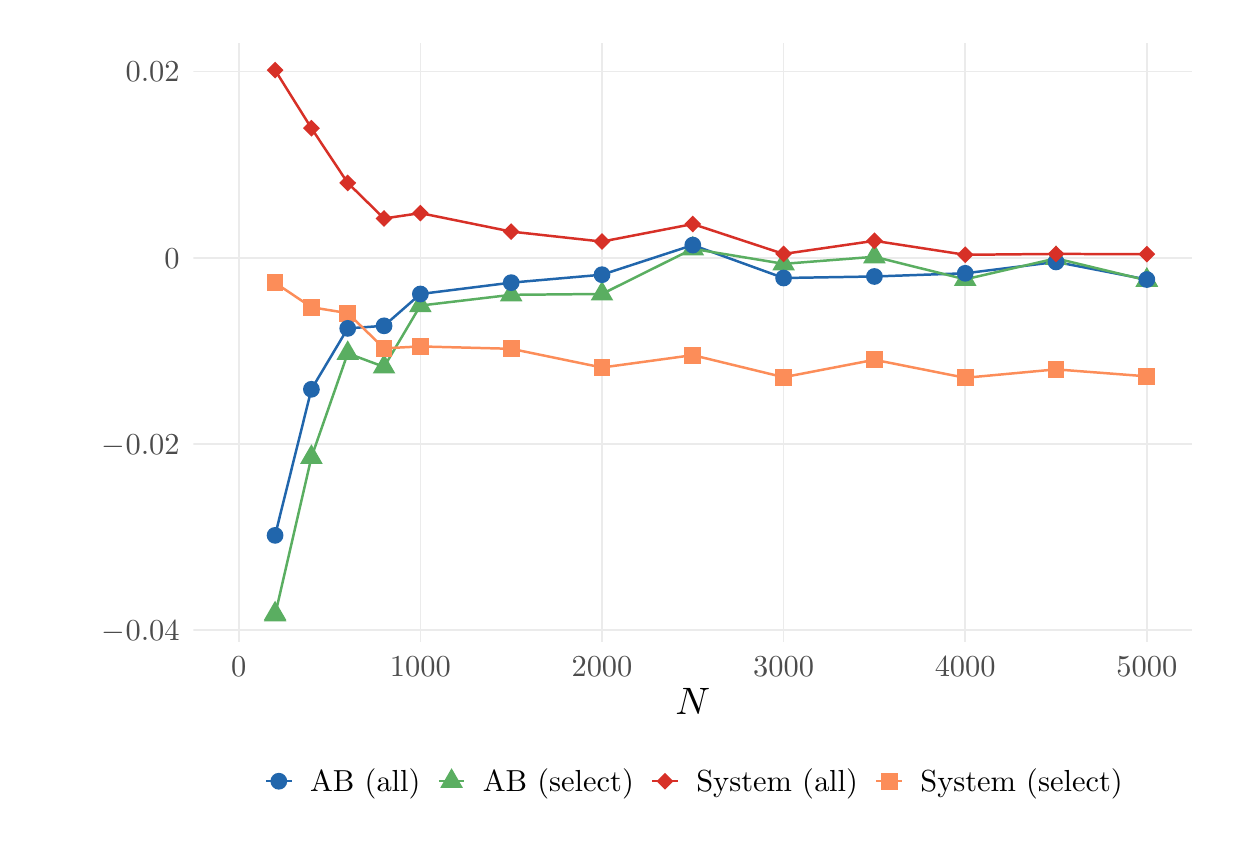
\begin{tikzpicture}[x=1pt,y=1pt]
\definecolor{fillColor}{RGB}{255,255,255}
\path[use as bounding box,fill=fillColor,fill opacity=0.00] (0,0) rectangle (433.62,289.08);
\begin{scope}
\path[clip] ( 59.87, 67.02) rectangle (420.81,283.58);
\definecolor{drawColor}{gray}{0.92}

\path[draw=drawColor,line width= 0.6pt,line join=round] ( 59.87, 71.38) --
	(420.81, 71.38);

\path[draw=drawColor,line width= 0.6pt,line join=round] ( 59.87,138.67) --
	(420.81,138.67);

\path[draw=drawColor,line width= 0.6pt,line join=round] ( 59.87,205.96) --
	(420.81,205.96);

\path[draw=drawColor,line width= 0.6pt,line join=round] ( 59.87,273.25) --
	(420.81,273.25);

\path[draw=drawColor,line width= 0.6pt,line join=round] ( 76.28, 67.02) --
	( 76.28,283.58);

\path[draw=drawColor,line width= 0.6pt,line join=round] (141.90, 67.02) --
	(141.90,283.58);

\path[draw=drawColor,line width= 0.6pt,line join=round] (207.53, 67.02) --
	(207.53,283.58);

\path[draw=drawColor,line width= 0.6pt,line join=round] (273.15, 67.02) --
	(273.15,283.58);

\path[draw=drawColor,line width= 0.6pt,line join=round] (338.78, 67.02) --
	(338.78,283.58);

\path[draw=drawColor,line width= 0.6pt,line join=round] (404.40, 67.02) --
	(404.40,283.58);
\definecolor{drawColor}{RGB}{33,102,172}

\path[draw=drawColor,line width= 0.9pt,line join=round] ( 89.40,105.62) --
	(102.53,158.41) --
	(115.65,180.42) --
	(128.78,181.34) --
	(141.90,192.84) --
	(174.72,196.94) --
	(207.53,199.81) --
	(240.34,210.52) --
	(273.15,198.62) --
	(305.97,199.17) --
	(338.78,200.32) --
	(371.59,204.42) --
	(404.40,198.07);
\definecolor{drawColor}{RGB}{90,174,97}

\path[draw=drawColor,line width= 0.9pt,line join=round] ( 89.40, 77.31) --
	( 89.40, 76.86) --
	(102.53,133.84) --
	(115.65,171.40) --
	(128.78,166.50) --
	(141.90,188.66) --
	(174.72,192.54) --
	(207.53,192.85) --
	(240.34,209.17) --
	(273.15,203.74) --
	(305.97,206.29) --
	(338.78,198.14) --
	(371.59,205.71) --
	(404.40,197.79) --
	(404.40,197.79);
\definecolor{drawColor}{RGB}{215,48,39}

\path[draw=drawColor,line width= 0.9pt,line join=round] ( 89.40,273.74) --
	(102.53,252.75) --
	(115.65,232.99) --
	(128.78,220.13) --
	(141.90,222.07) --
	(174.72,215.39) --
	(207.53,211.78) --
	(240.34,218.12) --
	(273.15,207.31) --
	(305.97,212.06) --
	(338.78,207.01) --
	(371.59,207.32) --
	(404.40,207.23);
\definecolor{drawColor}{RGB}{252,141,89}

\path[draw=drawColor,line width= 0.9pt,line join=round] ( 89.40,197.12) --
	( 89.40,196.90) --
	(102.53,188.06) --
	(115.65,185.92) --
	(128.78,173.21) --
	(141.90,173.89) --
	(174.72,173.04) --
	(207.53,166.27) --
	(240.34,170.75) --
	(273.15,162.77) --
	(305.97,169.07) --
	(338.78,162.56) --
	(371.59,165.60) --
	(404.40,163.09) --
	(404.40,163.09);
\definecolor{fillColor}{RGB}{90,174,97}

\path[fill=fillColor] (141.90,193.38) --
	(145.99,186.30) --
	(137.82,186.30) --
	cycle;
\definecolor{fillColor}{RGB}{252,141,89}

\path[fill=fillColor] (138.87,170.86) --
	(144.94,170.86) --
	(144.94,176.92) --
	(138.87,176.92) --
	cycle;
\definecolor{fillColor}{RGB}{90,174,97}

\path[fill=fillColor] (174.72,197.26) --
	(178.80,190.19) --
	(170.63,190.19) --
	cycle;
\definecolor{fillColor}{RGB}{252,141,89}

\path[fill=fillColor] (171.68,170.01) --
	(177.75,170.01) --
	(177.75,176.07) --
	(171.68,176.07) --
	cycle;
\definecolor{fillColor}{RGB}{90,174,97}

\path[fill=fillColor] ( 89.40, 82.02) --
	( 93.49, 74.95) --
	( 85.32, 74.95) --
	cycle;
\definecolor{fillColor}{RGB}{252,141,89}

\path[fill=fillColor] ( 86.37,194.09) --
	( 92.44,194.09) --
	( 92.44,200.15) --
	( 86.37,200.15) --
	cycle;
\definecolor{fillColor}{RGB}{90,174,97}

\path[fill=fillColor] ( 89.40, 81.58) --
	( 93.49, 74.50) --
	( 85.32, 74.50) --
	cycle;
\definecolor{fillColor}{RGB}{252,141,89}

\path[fill=fillColor] ( 86.37,193.87) --
	( 92.44,193.87) --
	( 92.44,199.94) --
	( 86.37,199.94) --
	cycle;
\definecolor{fillColor}{RGB}{90,174,97}

\path[fill=fillColor] (207.53,197.57) --
	(211.61,190.50) --
	(203.44,190.50) --
	cycle;
\definecolor{fillColor}{RGB}{252,141,89}

\path[fill=fillColor] (204.50,163.24) --
	(210.56,163.24) --
	(210.56,169.31) --
	(204.50,169.31) --
	cycle;
\definecolor{fillColor}{RGB}{90,174,97}

\path[fill=fillColor] (240.34,213.88) --
	(244.43,206.81) --
	(236.26,206.81) --
	cycle;
\definecolor{fillColor}{RGB}{252,141,89}

\path[fill=fillColor] (237.31,167.72) --
	(243.37,167.72) --
	(243.37,173.79) --
	(237.31,173.79) --
	cycle;
\definecolor{fillColor}{RGB}{90,174,97}

\path[fill=fillColor] (273.15,208.46) --
	(277.24,201.38) --
	(269.07,201.38) --
	cycle;
\definecolor{fillColor}{RGB}{252,141,89}

\path[fill=fillColor] (270.12,159.74) --
	(276.19,159.74) --
	(276.19,165.80) --
	(270.12,165.80) --
	cycle;
\definecolor{fillColor}{RGB}{90,174,97}

\path[fill=fillColor] (305.97,211.01) --
	(310.05,203.94) --
	(301.88,203.94) --
	cycle;
\definecolor{fillColor}{RGB}{252,141,89}

\path[fill=fillColor] (302.93,166.04) --
	(309.00,166.04) --
	(309.00,172.11) --
	(302.93,172.11) --
	cycle;
\definecolor{fillColor}{RGB}{90,174,97}

\path[fill=fillColor] (102.53,138.55) --
	(106.61,131.48) --
	( 98.44,131.48) --
	cycle;
\definecolor{fillColor}{RGB}{252,141,89}

\path[fill=fillColor] ( 99.50,185.02) --
	(105.56,185.02) --
	(105.56,191.09) --
	( 99.50,191.09) --
	cycle;
\definecolor{fillColor}{RGB}{90,174,97}

\path[fill=fillColor] (338.78,202.85) --
	(342.86,195.78) --
	(334.69,195.78) --
	cycle;
\definecolor{fillColor}{RGB}{252,141,89}

\path[fill=fillColor] (335.75,159.53) --
	(341.81,159.53) --
	(341.81,165.59) --
	(335.75,165.59) --
	cycle;
\definecolor{fillColor}{RGB}{90,174,97}

\path[fill=fillColor] (371.59,210.43) --
	(375.68,203.35) --
	(367.51,203.35) --
	cycle;
\definecolor{fillColor}{RGB}{252,141,89}

\path[fill=fillColor] (368.56,162.57) --
	(374.63,162.57) --
	(374.63,168.63) --
	(368.56,168.63) --
	cycle;
\definecolor{fillColor}{RGB}{90,174,97}

\path[fill=fillColor] (404.40,202.51) --
	(408.49,195.44) --
	(400.32,195.44) --
	cycle;
\definecolor{fillColor}{RGB}{252,141,89}

\path[fill=fillColor] (401.37,160.06) --
	(407.44,160.06) --
	(407.44,166.12) --
	(401.37,166.12) --
	cycle;
\definecolor{fillColor}{RGB}{90,174,97}

\path[fill=fillColor] (404.40,202.51) --
	(408.49,195.44) --
	(400.32,195.44) --
	cycle;
\definecolor{fillColor}{RGB}{252,141,89}

\path[fill=fillColor] (401.37,160.06) --
	(407.44,160.06) --
	(407.44,166.12) --
	(401.37,166.12) --
	cycle;
\definecolor{fillColor}{RGB}{90,174,97}

\path[fill=fillColor] (115.65,176.11) --
	(119.74,169.04) --
	(111.57,169.04) --
	cycle;
\definecolor{fillColor}{RGB}{252,141,89}

\path[fill=fillColor] (112.62,182.88) --
	(118.69,182.88) --
	(118.69,188.95) --
	(112.62,188.95) --
	cycle;
\definecolor{fillColor}{RGB}{90,174,97}

\path[fill=fillColor] (128.78,171.21) --
	(132.86,164.14) --
	(124.69,164.14) --
	cycle;
\definecolor{fillColor}{RGB}{252,141,89}

\path[fill=fillColor] (125.75,170.18) --
	(131.81,170.18) --
	(131.81,176.24) --
	(125.75,176.24) --
	cycle;
\definecolor{fillColor}{RGB}{33,102,172}

\path[fill=fillColor] (141.90,192.84) circle (  3.03);
\definecolor{fillColor}{RGB}{215,48,39}

\path[fill=fillColor] (138.87,222.07) --
	(141.90,225.11) --
	(144.94,222.07) --
	(141.90,219.04) --
	cycle;
\definecolor{fillColor}{RGB}{33,102,172}

\path[fill=fillColor] (174.72,196.94) circle (  3.03);
\definecolor{fillColor}{RGB}{215,48,39}

\path[fill=fillColor] (171.68,215.39) --
	(174.72,218.42) --
	(177.75,215.39) --
	(174.72,212.35) --
	cycle;
\definecolor{fillColor}{RGB}{33,102,172}

\path[fill=fillColor] ( 89.40,105.62) circle (  3.03);
\definecolor{fillColor}{RGB}{215,48,39}

\path[fill=fillColor] ( 86.37,273.74) --
	( 89.40,276.77) --
	( 92.44,273.74) --
	( 89.40,270.70) --
	cycle;
\definecolor{fillColor}{RGB}{33,102,172}

\path[fill=fillColor] (207.53,199.81) circle (  3.03);
\definecolor{fillColor}{RGB}{215,48,39}

\path[fill=fillColor] (204.50,211.78) --
	(207.53,214.82) --
	(210.56,211.78) --
	(207.53,208.75) --
	cycle;
\definecolor{fillColor}{RGB}{33,102,172}

\path[fill=fillColor] (240.34,210.52) circle (  3.03);
\definecolor{fillColor}{RGB}{215,48,39}

\path[fill=fillColor] (237.31,218.12) --
	(240.34,221.15) --
	(243.37,218.12) --
	(240.34,215.08) --
	cycle;
\definecolor{fillColor}{RGB}{33,102,172}

\path[fill=fillColor] (273.15,198.62) circle (  3.03);
\definecolor{fillColor}{RGB}{215,48,39}

\path[fill=fillColor] (270.12,207.31) --
	(273.15,210.34) --
	(276.19,207.31) --
	(273.15,204.28) --
	cycle;
\definecolor{fillColor}{RGB}{33,102,172}

\path[fill=fillColor] (305.97,199.17) circle (  3.03);
\definecolor{fillColor}{RGB}{215,48,39}

\path[fill=fillColor] (302.93,212.06) --
	(305.97,215.09) --
	(309.00,212.06) --
	(305.97,209.03) --
	cycle;
\definecolor{fillColor}{RGB}{33,102,172}

\path[fill=fillColor] (102.53,158.41) circle (  3.03);
\definecolor{fillColor}{RGB}{215,48,39}

\path[fill=fillColor] ( 99.50,252.75) --
	(102.53,255.78) --
	(105.56,252.75) --
	(102.53,249.71) --
	cycle;
\definecolor{fillColor}{RGB}{33,102,172}

\path[fill=fillColor] (338.78,200.32) circle (  3.03);
\definecolor{fillColor}{RGB}{215,48,39}

\path[fill=fillColor] (335.75,207.01) --
	(338.78,210.05) --
	(341.81,207.01) --
	(338.78,203.98) --
	cycle;
\definecolor{fillColor}{RGB}{33,102,172}

\path[fill=fillColor] (371.59,204.42) circle (  3.03);
\definecolor{fillColor}{RGB}{215,48,39}

\path[fill=fillColor] (368.56,207.32) --
	(371.59,210.35) --
	(374.63,207.32) --
	(371.59,204.29) --
	cycle;
\definecolor{fillColor}{RGB}{33,102,172}

\path[fill=fillColor] (404.40,198.07) circle (  3.03);
\definecolor{fillColor}{RGB}{215,48,39}

\path[fill=fillColor] (401.37,207.23) --
	(404.40,210.27) --
	(407.44,207.23) --
	(404.40,204.20) --
	cycle;
\definecolor{fillColor}{RGB}{33,102,172}

\path[fill=fillColor] (115.65,180.42) circle (  3.03);
\definecolor{fillColor}{RGB}{215,48,39}

\path[fill=fillColor] (112.62,232.99) --
	(115.65,236.02) --
	(118.69,232.99) --
	(115.65,229.95) --
	cycle;
\definecolor{fillColor}{RGB}{33,102,172}

\path[fill=fillColor] (128.78,181.34) circle (  3.03);
\definecolor{fillColor}{RGB}{215,48,39}

\path[fill=fillColor] (125.75,220.13) --
	(128.78,223.17) --
	(131.81,220.13) --
	(128.78,217.10) --
	cycle;
\end{scope}
\begin{scope}
\path[clip] (  0.00,  0.00) rectangle (433.62,289.08);
\definecolor{drawColor}{gray}{0.30}

\node[text=drawColor,anchor=base east,inner sep=0pt, outer sep=0pt, scale=  1.10] at ( 54.92, 67.59) {$-0.04$};

\node[text=drawColor,anchor=base east,inner sep=0pt, outer sep=0pt, scale=  1.10] at ( 54.92,134.88) {$-0.02$};

\node[text=drawColor,anchor=base east,inner sep=0pt, outer sep=0pt, scale=  1.10] at ( 54.92,202.17) {$0$};

\node[text=drawColor,anchor=base east,inner sep=0pt, outer sep=0pt, scale=  1.10] at ( 54.92,269.46) {$0.02$};
\end{scope}
\begin{scope}
\path[clip] (  0.00,  0.00) rectangle (433.62,289.08);
\definecolor{drawColor}{gray}{0.30}

\node[text=drawColor,anchor=base,inner sep=0pt, outer sep=0pt, scale=  1.10] at ( 76.28, 54.49) {$0$};

\node[text=drawColor,anchor=base,inner sep=0pt, outer sep=0pt, scale=  1.10] at (141.90, 54.49) {$1000$};

\node[text=drawColor,anchor=base,inner sep=0pt, outer sep=0pt, scale=  1.10] at (207.53, 54.49) {$2000$};

\node[text=drawColor,anchor=base,inner sep=0pt, outer sep=0pt, scale=  1.10] at (273.15, 54.49) {$3000$};

\node[text=drawColor,anchor=base,inner sep=0pt, outer sep=0pt, scale=  1.10] at (338.78, 54.49) {$4000$};

\node[text=drawColor,anchor=base,inner sep=0pt, outer sep=0pt, scale=  1.10] at (404.40, 54.49) {$5000$};
\end{scope}
\begin{scope}
\path[clip] (  0.00,  0.00) rectangle (433.62,289.08);
\definecolor{drawColor}{RGB}{0,0,0}

\node[text=drawColor,anchor=base,inner sep=0pt, outer sep=0pt, scale=  1.38] at (240.34, 40.85) {$N$};
\end{scope}
\begin{scope}
\path[clip] (  0.00,  0.00) rectangle (433.62,289.08);
\definecolor{drawColor}{RGB}{33,102,172}

\path[draw=drawColor,line width= 0.9pt,line join=round] ( 86.12, 16.78) -- ( 95.37, 16.78);
\end{scope}
\begin{scope}
\path[clip] (  0.00,  0.00) rectangle (433.62,289.08);
\definecolor{fillColor}{RGB}{33,102,172}

\path[fill=fillColor] ( 90.75, 16.78) circle (  3.03);
\end{scope}
\begin{scope}
\path[clip] (  0.00,  0.00) rectangle (433.62,289.08);
\definecolor{drawColor}{RGB}{90,174,97}

\path[draw=drawColor,line width= 0.9pt,line join=round] (148.55, 16.78) -- (157.80, 16.78);
\end{scope}
\begin{scope}
\path[clip] (  0.00,  0.00) rectangle (433.62,289.08);
\definecolor{fillColor}{RGB}{90,174,97}

\path[fill=fillColor] (153.18, 21.50) --
	(157.26, 14.42) --
	(149.09, 14.42) --
	cycle;
\end{scope}
\begin{scope}
\path[clip] (  0.00,  0.00) rectangle (433.62,289.08);
\definecolor{drawColor}{RGB}{215,48,39}

\path[draw=drawColor,line width= 0.9pt,line join=round] (225.71, 16.78) -- (234.96, 16.78);
\end{scope}
\begin{scope}
\path[clip] (  0.00,  0.00) rectangle (433.62,289.08);
\definecolor{fillColor}{RGB}{215,48,39}

\path[fill=fillColor] (227.30, 16.78) --
	(230.33, 19.81) --
	(233.36, 16.78) --
	(230.33, 13.75) --
	cycle;
\end{scope}
\begin{scope}
\path[clip] (  0.00,  0.00) rectangle (433.62,289.08);
\definecolor{drawColor}{RGB}{252,141,89}

\path[draw=drawColor,line width= 0.9pt,line join=round] (306.68, 16.78) -- (315.93, 16.78);
\end{scope}
\begin{scope}
\path[clip] (  0.00,  0.00) rectangle (433.62,289.08);
\definecolor{fillColor}{RGB}{252,141,89}

\path[fill=fillColor] (308.27, 13.75) --
	(314.34, 13.75) --
	(314.34, 19.81) --
	(308.27, 19.81) --
	cycle;
\end{scope}
\begin{scope}
\path[clip] (  0.00,  0.00) rectangle (433.62,289.08);
\definecolor{drawColor}{RGB}{0,0,0}

\node[text=drawColor,anchor=base west,inner sep=0pt, outer sep=0pt, scale=  1.10] at (102.03, 12.99) {AB (all)};
\end{scope}
\begin{scope}
\path[clip] (  0.00,  0.00) rectangle (433.62,289.08);
\definecolor{drawColor}{RGB}{0,0,0}

\node[text=drawColor,anchor=base west,inner sep=0pt, outer sep=0pt, scale=  1.10] at (164.46, 12.99) {AB (select)};
\end{scope}
\begin{scope}
\path[clip] (  0.00,  0.00) rectangle (433.62,289.08);
\definecolor{drawColor}{RGB}{0,0,0}

\node[text=drawColor,anchor=base west,inner sep=0pt, outer sep=0pt, scale=  1.10] at (241.61, 12.99) {System (all)};
\end{scope}
\begin{scope}
\path[clip] (  0.00,  0.00) rectangle (433.62,289.08);
\definecolor{drawColor}{RGB}{0,0,0}

\node[text=drawColor,anchor=base west,inner sep=0pt, outer sep=0pt, scale=  1.10] at (322.58, 12.99) {System (select)};
\end{scope}
\end{tikzpicture}
